% !TEX root = ../thesis.tex

\chapter{MATLAB WPS}
\label{sec:matlabwps}

MATLAB \citep{matlabproduct} is a closed source, commercial software by The MathWorks, Inc. for numerical computation, visualization and programming. It features a high-level programming language as well as an cross-platform (Windows, Linux and Mac OS X) interactive desktop environment. Initially developed for matrix computations \citep[hence \emph{MAT}rix \emph{LAB}oratory,][]{matlabhistory}, today MATLAB is widespread across different domains in academics, engineering and industry. The base program is extensible by using so called \emph{toolboxes}, which add functionalities for various domains, like statistics, curve fitting, neural networks, image processing, economics, bioinformatics or signal processing. Besides that, functions, algorithms, files or toolboxes can be installed through \emph{MATLAB Central}, a repository of user contributions. These are licensed under the 2-clause \citep{bsd2} or 3-clause \citep{bsd3} BSD license \citep{matlabtransitionfaq}.

Creating a specific \ac{WPS} process implementation for the \la would be possible. Considering the wide spread usage of MATLAB-based scripts and applications, a generic solution that enables the easy deployment of MATLAB-based functionalities as \ac{WPS} processes would have a huge benefit for the geospatial community as well as for the the acceptance of the \ac{WPS} across disciplines. A generic \emph{MATLAB WPS} would not only open the \la for an interoperable usage in existing web processing chains, but would also make existing models and algorithms implemented in MATLAB instantly available to a larger audience and can increase reusability of software components and exchange between different areas of research, development and business. Considering the diversified fields MATLAB is used in, a software component such as a MATLAB WPS can not assume an extensive programming experience beyond MATLAB. Domain experts developing models or algorithms in MATLAB should be able to offer a MATLAB script or function as a \ac{WPS} process using a simple and straightforward procedure, without any knowledge of other programming languages or a comprehensive expertise in web services or their development. To accomplish this, a switch from MATLAB to other languages should not be required, and rather complex and verbose process descriptions should not be manually be written, but automatically generated. A key goal of the MATLAB WPS is to expose existing models and algorithms as \ac{WPS} processes. Therefore, the procedure to convert a MATLAB script or function should not require intrusive changes to be compatible with the MATLAB WPS.

Approaches to offer data analysis and modeling languages like MATLAB as \ac{WPS} processes do already exist. Specially emphasized should be the \emph{WPS4R} \citep{wps4r} project that creates WPS processes from scripts written for the statistical analysis environment \emph{R} \citep{gnur}. Written as a module for the \ftn \ac{WPS} implementation, it shares many requirements and challenges with a MATLAB WPS. R is also an environment used mostly by domain experts and features a massive amount of existing models and algorithm implementations. These are worth to be opened to the web processing environment and to be made available to a broader user base using interoperable standards like the \ac{OGC} \acl{WPS}.

\lstinputlisting[label={lst:r:annotation},
         caption={[Example for a comment containing annotations used by WPS4R.]Example for a comment containing annotations used by WPS4R \citep{wps4r}.},
         language=R]{listings/wps4r-annotations.r}

WPS4R takes an R script and executes it on a remote or local R instance using \emph{Rserve} \citep{rserve}. In contrast to the \ac{WPS} interface which explicitly states types of input and output parameters to allow service discovery and the usage of generic clients, R is a weakly and dynamically typed language. By this, the \ac{WPS} is not able to parse the script and determine appropriate input and output parameter types, as these are only available at runtime. To bind static types to input and output parameters, an annotation mechanism was developed which is also capable to detail input/output and process meta data. In contrast to other programming languages, like Java \citep{jsr175} or C\# \citep{ecma335}, R does not feature a native annotation mechanism. Because of this, the annotations are encoded as comments featuring special keywords (\emph{wps.in}, \emph{wps.out} and \emph{wps.des}), followed by a key value list representing the necessary information to generate a process description (see \cref{lst:r:annotation}). During process execution, WPS4R will populate the described input parameter variables using \ac{WPS} inputs, execute the script, read the specified output variables from the R session and transform them to WPS outputs. The usage of annotations embedded in comments support the deployment of R functionalities as WPS processes by providing a single script file that the WPS4R can parse.

Literal input parameters are translated into native R types, whereas complex inputs are transferred as files to a temporary working directory. Complex input and output parameters need to be described by a single keyword, denoting the mime type of the parameter, which that has to be registered to WPS4R using a configuration file. Describing complex inputs and outputs using \emph{schema} or \emph{encoding}, or using any mime type without changing the WPS4R configuration, is not possible. This may be caused by the reduced expressiveness through the usage of a structureless description format (e.g. denoting multiple supported complex input formats, would be hard to specify). Scripts are run on globally configured Rserve connections. Different remotes for different processes or a load balancing between multiple remote nodes running R are not possible. Furthermore, the easy deployment of scripts consisting of multiple files is currently not possible.

The comment-based approach taken by WPS4R has several advantages like having \ac{WPS} configuration and actual code side by side (which results in less maintenance effort), but also introduces considerable drawbacks, especially if the annotation mechanism should be applied to MATLAB. Conveying important information in comments can be problematic. Even though there are many examples where comments are used (e.g. to generate documentation as seen on the example of Javadoc \citep{javadoc}), these are often standardized at language level or include a large user base and a wide support in editors and development environments. The syntax of a custom comment-based annotation mechanism as used in this approach, can not be verified in editors or interpreters. By this and the unstructured notation of comments, the approach becomes heavily prone to user error, which can not be detected before the deployment to a WPS instance. Additionally, annotations are not actually bound to any language construct, but just happen to be in the same file.

Typical MATLAB programs would not benefit from combining annotations and scripts in a single file, as it is common practice -- or even a requirement to access a function from outside -- to place a function in its own file. By this, MATLAB programs tend to consist of multiple files, and can not easily deployed as single script files.

In contrast to R, MATLAB offers multiple return values of functions as a native language feature (see \cref{lst:matlab:example:fun}). Through this, MATLAB functions are able to directly represent a \ac{WPS} process, and the MATLAB WPS should use MATLAB functions instead of scripts to offer functionalities as WPS processes. As stated before, MATLAB is a weakly and dynamically typed language, and the parsing of a function signature can not create a statically typed binding as the \ac{WPS} standard requires. For this, an additional description mechanism needs to be developed that allows the semi-automatically generation of process descriptions. This should be done without extensive knowledge of web service development or programming languages. Also the deployment of existing MATLAB functions should be a straightforward non-intrusive process. Similar to R, MATLAB instances are single threaded, and so can only process one WPS process execution a time. Moreover, and contrary to R, opening the MATLAB workbench even in a headless mode (i.e. without any user interface) can take considerable time. This requires an efficient usage of MATLAB instances, especially the reuse of already started MATLAB instances to reduce latency of process executions. Complex inputs should be usable inside of MATLAB without restrictions to any format, and without the need to change any configuration files.

\lstinputlisting[label={lst:matlab:example:fun},
         caption={MATLAB example function that calculates statistical characteristics (mean and standard deviation) of an input vector.},
         language=Matlab]{listings/matlab-stat-function.m}

This chapter will outline the conceptualization and implementation of a MATLAB WPS by describing its architecture and configuration mechanism. Furthermore, details of the conversion between MATLAB and WPS types will be discussed and legal implications of offering commercial software as web services will be shortly examined. Finally, the generic capabilities of the MATLAB WPS will be used in order to offer the \la as a WPS process.

\section{Architecture}
  The MATLAB WPS features a multi-tier architecture to offer MATLAB functions as \acl{WPS} processes. A detailed sequence diagram depicting a MATLAB WPS process execution can be seen in \cref{fig:sd:mwps}. An incoming WPS \emph{Execute} request is accepted by the MATLAB WPS (\step{fig:sd:mwps}{1}). The \emph{Execute} request is verified (e.g. no missing inputs, inputs within the range described by the process description, etc.) and then translated into a MATLAB request (\step{fig:sd:mwps}{2}). This request is send via a WebSocket connection to a configured MATLAB server (\step{fig:sd:mwps}{3}). The MATLAB server maintains a pool of MATLAB instances and will dispatch the request to one of these as soon as one becomes available (\step{fig:sd:mwps}{4}). The instance transforms the MATLAB request into MATLAB syntax (\step{fig:sd:mwps}{5}) and evaluates the MATLAB command in an associated MATLAB session. After this (\step{fig:sd:mwps}{6}), the return values are read from the session (\step{fig:sd:mwps}{7}) and encoded as a MATLAB response (\step{fig:sd:mwps}{8}). It is then passed through the MATLAB server (\step{fig:sd:mwps}{9}) to the MATLAB WPS (\step{fig:sd:mwps}{10}). The MATLAB WPS process translates the MATLAB response to a WPS \emph{Execute} response (\step{fig:sd:mwps}{11}) and returns it to the client (\step{fig:sd:mwps}{12}).

  \begin{figure}[!htb]
    \centering
    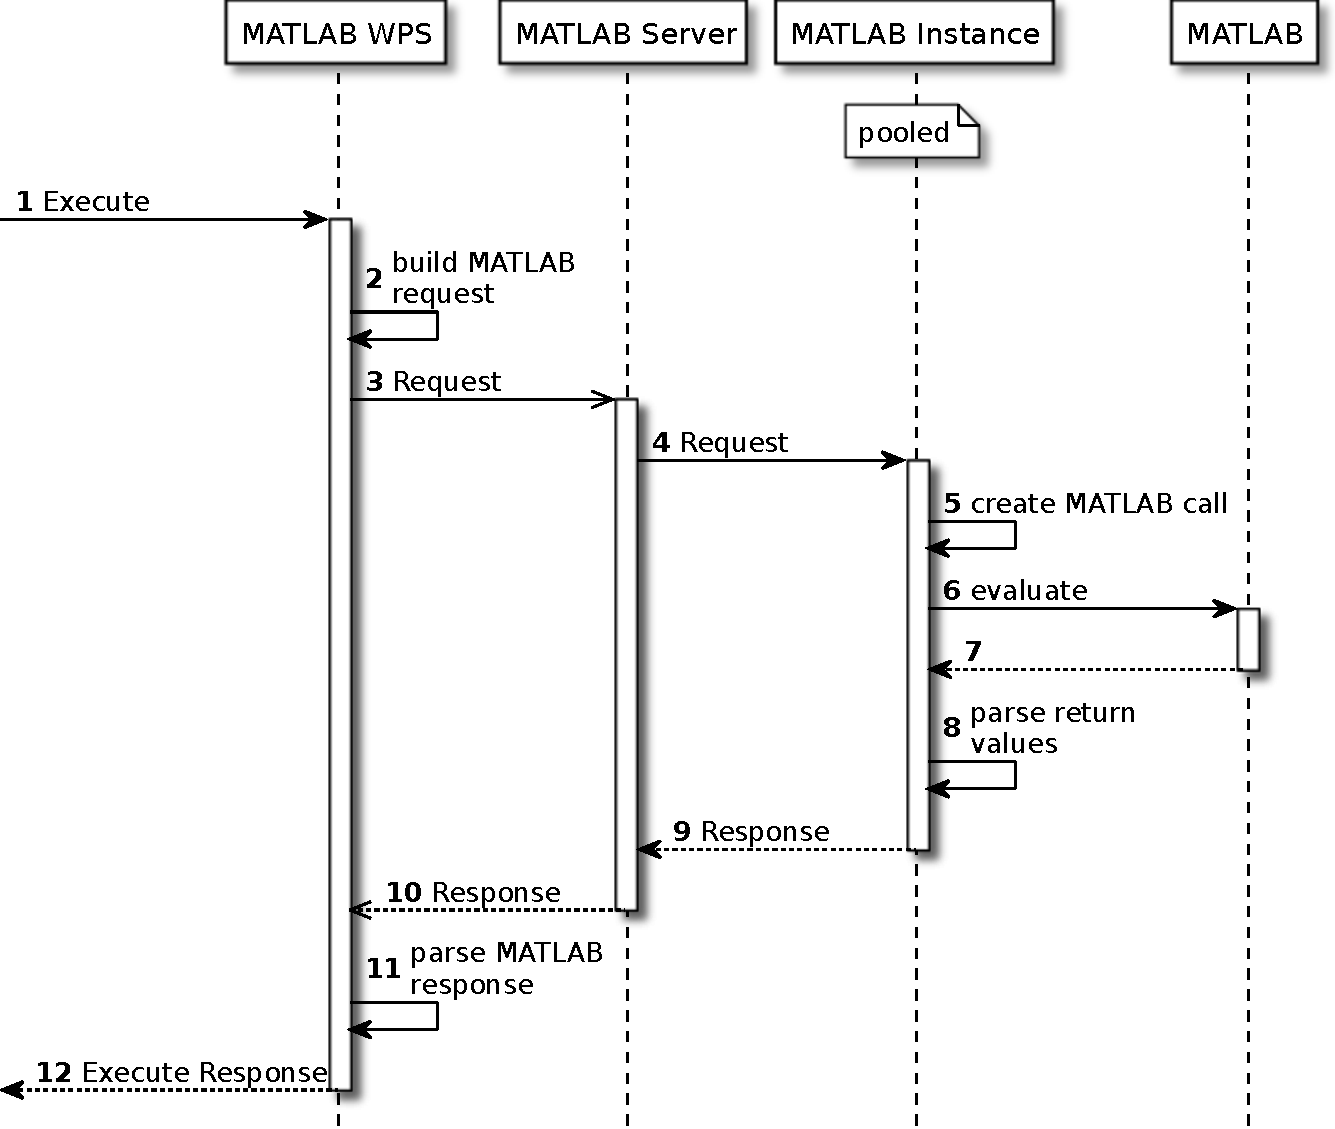
\includegraphics[width = 0.6788732394366197\linewidth]{figures/sequence-diagram-mwps.pdf}
    \caption{\label{fig:sd:mwps}Sequence diagram of a MATLAB WPS process execution.}
  \end{figure}

  Besides an option to run the MATLAB server locally, all communication between the MATLAB WPS and MATLAB server is done over WebSockets \citep{ietf:rfc6455}. WebSockets are defining a TCP-based protocol that creates a bidirectional communication channel between client and server. A primary goal of WebSockets is to bring the benefits of efficient full-duplex communication to the web browser environment. This is accomplished by an HTTP compatible socket initiation mechanism (see \cref{lst:websocket}). A client opens a new WebSocket by issuing an HTTP request to the server, in which it requires an upgrade to the WebSocket protocol. Afterwards, the connection is kept open and both client and server can send messages to the opposing party. These messages are transported using one or more text or binary frames and allow an efficient bidirectional information exchange. By using HTTP for the initial handshake, WebSockets can be used in most proxy setups and despite the presence of firewalls that filter non HTTP traffic and can facilitate HTTP's access control mechanisms and client side security measures like \acl{CORS} \citep[\acs{CORS},][]{w3c:cors}.

  \lstinputlisting[caption={[WebSocket opening handshake using a HTTP upgrade request.]WebSocket opening handshake using a HTTP upgrade request \citep{ietf:rfc6455}.},label={lst:websocket}]{listings/websocket-handshake.txt}

  Even though the opening handshake is using HTTP, WebSockets do not conform to the HTTP protocol. To ensure that a web server can handle WebSocket connections, the client sends the header \emph{Sec-WebSocket-Key} in the opening request, containing 16 bytes of random data in base 64 encoding \citep{ietf:rfc4648}. The server has to append the Globally Unique Identifier \cite[GUID,][]{ietf:rfc4122} \emph{258EAFA5-E914-47DA-95CA-C5AB0DC85B11} to the header value and return the base 64 encoded SHA-1 \citep{NistFIPS1803} hash sum using the \emph{Sec-WebSocket-Accept} header field. Because of the incompatibility with the HTTP protocol, WebSockets define two separate URL schemes: \emph{ws} for normal WebSocket connections and \emph{wss} for secure WebSocket connection, which resemble the HTTP and HTTPS protocol and share their default ports 80 and 443.

  The WebSocket protocol is accompanied with an HTML5 JavaScript \ac{API} \citep{w3c:ws} that is implemented in all recent versions of major desktop browsers\footnote{And with the exception of Opera Mini also mobile browsers.} \citep{caniuse}. Besides that, WebSocket client and server implementations for nearly all programming languages exist, e.g.
  R \citep{websocketr}, C \citep{websocketc}, C\# \citep{websocketcsharp} or Java \citep{jsr356}.

  As previously noted, function calls are used as the central element of MATLAB WPS processes. Using the native language feature of multiple return values, WPS processes can be represented as MATLAB functions one to one. The MATLAB WPS is not designed to easily interface MATLAB with the WPS implementation to allow process development from within the WPS, but to allow the deployment of any MATLAB model using a WPS. Because of this, the MATLAB WPS only offers functionalities to evaluate a single function call and is not required to evaluate scripts, parse MATLAB code or maintain variable references. By this, a very thin implementation is possible and the configuration and maintenance efforts are reduced to a minimum.

  The components \emph{MATLAB server} and \emph{MATLAB instance} as shown in \cref{fig:sd:mwps} are developed separately from the MATLAB WPS and can be easily used in other contexts. This \emph{matlab-connector}\footnote{The matlab-connector was initially developed for the UncertWeb project (\url{http://www.uncertweb.org/}), but was heavily extended for this thesis.} consists of a small Java CLI application (the server) and an associated Java client library used in the MATLAB WPS, which offers a simple \ac{API} to build MATLAB requests. The server component is started on the machine on which MATLAB is installed, and then offers a configurable amount of headless MATLAB instances using a small WebSocket server. The MATLAB instance communicates with a \ac{JVM} exposed by the MATLAB program using a Java \ac{RMI} wrapper called \emph{matlabcontrol} \citep{matlabcontrol}. As previously noted, MATLAB instances are, even in headless mode, heavy weight applications that require a considerable amount of resources and time to start. MATLAB instances are created at server startup and then are used to process requests. By reusing and preallocating a fixed amount of instances, the pooling of MATLAB instances reduces latency for WPS processes and saves resources on the server machine.

\section{Configuration}
  \label{sec:matlab:conf}
  Because of the aforementioned problems regarding comment annotations, the MATLAB WPS features another configuration mechanism. Process configurations are conveyed using YAML \citep{yaml} which facilitate a particular human-readable syntax. It allows easy structuring of data without delimiters like quotation marks or braces, but allows these e.g. to enable a more compact syntax. The structure of YAML has close resemblance with JSON (which is actually a valid subset of YAML since version 1.2) and features the same basic types of scalars, sequences and associative arrays (maps), but has additional features that make it more expressive. This includes comments, multi-line strings, references, multi-document files, sets, complex key types for maps, ordered/unordered maps and maps that allow duplicate keys.
  \lstinputlisting[language=YAML,
           label={lst:matlab:example:yaml},
           caption={MATLAB process configuration describing the function in \cref{lst:matlab:example:fun}.},
           morekeywords={function,connection,identifier,version,inputs,outputs,type,maxOccurs,title,abstract}]{listings/matlab-stat-process-configuration.yaml}
  Configuration files for the MATLAB WPS can contain multiple process configurations expressed as an associative array. These are describing a MATLAB function, their input and outputs as well as where the function should be executed. It resembles the basic structure of a WPS process description while concealing the verbosity and complexity of XML. \cref{lst:matlab:example:yaml} shows an example process configuration for the function displayed in \cref{lst:matlab:example:fun}. The process description generated from the YAML configuration can be found in \cref{lst:matlab:example:desc}.

  \lstinputlisting[label={lst:matlab:example:desc},
           caption={[Process description generated from the configuration in \cref{lst:matlab:example:yaml}.]Process description generated from the configuration in \cref{lst:matlab:example:yaml} (see \cref{sec:xmlnamespaces} for omitted XML namespaces).},
           language=XML]{listings/matlab-stat-process-description.xml}
  Top level attributes are describing the process itself, whereas \emph{inputs} holds a sequence of input descriptions and \emph{outputs} a sequence of output descriptions in the very same order the function is defined. The function to describe is denoted by the keyword \emph{function}. \emph{identifier}, \emph{title} and \emph{description} are directly mapped to their equivalent in the \ac{OGC} name space. The attribute \emph{maxOccurs} holds either an integral number or the special value \emph{unbounded} which will be translated to the platform specific maximum possible value (typically the greatest possible integer value). Data types, described under the keyword \emph{type}, are translated to their respective XML data type. Complex data types can be described using a map,generic containing a combination of \emph{mimeType}, \emph{schema} and \emph{encoding}. Bounding box inputs are described using a map containing the keyword \emph{crs}, which holds one or more supported \ac{CRS}.

  The attribute \emph{connection} denotes how the function should be executed. The keyword \emph{local} will cause the MATLAB WPS to start a pool of MATLAB instance in the current working directory. The function needs to be either at this path or at any other path searched by MATLAB. Other possible values for \emph{connection} are URIs in the \emph{ws}, \emph{wss} or \emph{file} scheme. The latter will start a connection pool inside the specified directory, while a WebSocket URL will cause the MATLAB WPS to connect to the remote server and will run the function there. In both cases, the file containing the function needs to be able to be found in the MATLAB search path.

  Through the very clear and concise YAML notation, complex process description can be easily written in a human readable format, which is way easier to maintain than custom annotations in inline comments. It results in a less error prone procedure for unexperienced domain experts, whereas advanced users are able to benefit from advanced YAML features. Furthermore, future enhancements and additions can be easily implemented backwards compatible.

\section{Type Mapping}
  \label{sec:matlab:type}
  MATLAB, like any other language, has a wide variety of data types. These include numeric types -- floating point numbers in single (\unit{32}{\bit}) and double (\unit{64}{\bit}) precision and signed and unsigned integers in \unit{8, 16, 32 and 64}{\bit} size -- logical, character/string types as well as structures, tables, cell arrays and function handles. Except for the latter, all of these types have the form of (possible multidimensional) arrays \citep{matlabdoc}.

  As previously described, the \acl{WPS} specification knows three different types of data: literal, complex and bounding box data. \ac{WPS} Literal data is mostly converted to their respective native MATLAB data type, but due to limitations in the MATLAB \ac{API}, this is not always possible. The \ac{API} exposed by MATLAB transfers every numerical type as floating point numbers of double precision. By this, an efficient handling of other basic data types like integral numbers or single precision floating point numbers is not possible. Within the WPS specification and implementation, these data types are each handled differently, but due to the limitations exposed by the MATLAB interface, MATLAB processes need to reduce precision on their own in order to reduce memory usage.

  Single and multiple occurrences of input parameters can be handled in MATLAB in the very same way, because every basic data type consists not only of a single value, but an array of its type. The sole exception are string-based data types, which are represented as an array of characters. Placing several strings in an array results in a concatenated string and so a MATLAB \emph{cell} is used for these data types. Boolean values are represented as \emph{logical} 0 or 1 or a respective array, and time stamp values are converted to their numerical representation\footnote{A double value containing the fractional number of days since the January 0, 0000.}.

  Bounding box input data is mapped to a \emph{struct} consisting of the fields \emph{crs} and \emph{bbox}, holding the \ac{CRS} identifier and a two-dimensional array with the upper and lower corner of the bounding box respectively. This format is also expected for bounding box outputs.

  Complex data is neither parsed nor converted using the MATLAB WPS. It is transferred to a temporary file and passed to the MATLAB function as a file name. For complex outputs, the MATLAB function saves them to a temporary file and returns the file name. The file is read by the MATLAB WPS and deleted when the process finishes. By delegating the parsing of complex data inputs to the MATLAB function, the WPS is independent from specific data formats -- both in case of specific MATLAB classes and in case of different XML or binary encodings at the WPS end -- and can easily be adopted to existing MATLAB models.

  The usage of complex outputs is currently limited to a single format. Even though the WPS specification allows the request of different formats (e.g. a raster or image can be requested as PNG, JPEG or TIFF, or a feature collection may be requested in different XML schemata), the MATLAB WPS does not offer this feature to MATLAB processes. This is owed to the MATLAB-based handling of complex inputs. To become independent of file formats and encodings, the MATLAB WPS can not be used to transform inputs or outputs between different formats. While the inputs and outputs of different format still could be created and consumed on the MATLAB process side, this possibility was neglected to ease MATLAB process development and to allow a more simple transformation of existing MATLAB models.

  MATLAB lacks a value to represent the absence of a value (often denoted as \emph{null}, \emph{nil}, \emph{none} or \emph{nothing} in other programming languages). Even though MATLAB supports optional parameters in function calls, it does not support named function parameters, and a function can only interpret the amount of input parameters to determine if an optional parameter is present or not. As WPS processes can contain a multitude of optional input parameters, the value \emph{NaN} \citep{ieee:754:2008}, which represents an undefined or unrepresentable numeric value and so comes close to a null value, is used to transport absent optional input parameters, regardless of their type.

  The WPS specification offers the possibility to only request specific outputs of a process. This enables the process to only compute the outputs that are really needed and thus can reduce the time needed for process executions. The MATLAB WPS currently does not support this mechanism and MATLAB functions are required to compute all outputs regardless which are requested by a client.
  %%% move this somewhere else?
  To overcome this issue, the requested output identifiers could be saved in a globally accessible environment variable. In addition to this, other contextual information could be conveyed using this method, e.g. the WPS service URL, which was used to execute the process or other meta data that the function may use.

  % !TEX root = ../thesis.tex

\begin{table}[!htb]
  \sffamily
  \centering
  \caption[Mapping between WPS data types and MATLAB types.]{\label{tab:matlab:typemapping}Mapping between WPS data types and MATLAB types. Absent optional parameters are denoted by \emph{NaN} ($1\times1$).}
  \begin{tabular}{@{}llcc@{}}
    \toprule\toprule
    &
    & \multicolumn{2}{b}{MATLAB Type}\\
    &
    & \multicolumn{1}{b}{Single}
    & \multicolumn{1}{b@{}}{Multiple}\\
    \midrule
    \multicolumn{2}{@{}l}{\textbf{Complex Data}}
    & char ($1\times{}m$)
    & cell of chars ($1\times{}n$)
    \\
    \midrule
    \multicolumn{2}{@{}l}{\textbf{Bounding Box Data}} & struct ($1\times1$) & cell of structs ($1\times{}n$)\\
    \midrule
    \textbf{Literal Data}
    & xs:string
    & \multirow{2}{*}{char ($1\times{}m$)}
    & \multirow{2}{*}{cell of chars ($1\times{}n$)}\\
    & xs:anyURI\\
    \cmidrule(r){2-4}
    & xs:byte
    & \multirow{7}{*}{double ($1\times1$)}
    & \multirow{7}{*}{double ($1\times{}n$)} \\
    & xs:short\\
    & xs:int\\
    & xs:long\\
    & xs:integer\\
    & xs:double\\
    & xs:float\\
    \cmidrule(r){2-4}
    & xs:boolean & logical ($1\times1$) & logical ($1\times{}n$) \\
    \cmidrule(r){2-4}
    & xs:dateTime & double/datenum ($1\times1$) & double/datenum ($1\times{}n$)\\
    \bottomrule\bottomrule
  \end{tabular}
\end{table}

  A list of literal \citep[based on][]{w3c:xmldatatypes}, bounding box and complex data types and their mapping to MATLAB types can be seen in \cref{tab:matlab:typemapping}. Structured data like structs, multidimensional arrays, cells or other objects can not be used as process outputs or inputs, as the \ac{WPS} specification lacks support for such types. A MATLAB process has to create a XML application schema or transform the structures to another file-based data typed that can be transported as WPS complex outputs.

\section{License Issues}
  MATLAB usage is, as any software, restricted by the software's license. MATLAB is a proprietary and commercial product and as such, the software and its usage is more restricted than e.g. an open source software such as the R Project. Relevant for the MATLAB WPS is section 4.8 of \emph{The MathWorks, Inc. Software License Agreement} \citep{matlablicense}:
  \begin{xquote}\itshape\small
    ``4. LICENSE RESTRICTIONS. The License is subject to the express restrictions
    set forth below. Licensee shall not, and shall not permit any Affiliate or any
    Third Party to:
      [...]
      4.8. provide access (directly or indirectly) to the Programs via a web or
      network Application, except as permitted in Article 8 of the Deployment
      Addendum;''
  \end{xquote}

  As the MATLAB WPS offers MATLAB functionalities through a web service interface, the usage is highly restricted, as the referenced \emph{Deployment Addendum} (ibidem) states:

  \begin{xquote}\itshape\small
    ``8. WEB APPLICATIONS. Licensee may not provide access to an entire Program or a substantial portion of a Program by means of a web interface.

    For the Network Concurrent User Activation Type. Programs licensed under the Network Concurrent User Activation Type may be called via a web application, provided the web application does not provide access to the MATLAB command line, or any of the licensed Programs with code generation capabilities. In addition, Licensed Users may not provide access to an entire Program or a substantial portion of a Program. Such operation of an application via a web interface may be provided to an unlimited number of web browser clients, at no additional cost, for Licensee's own use for its Internal Operations, and for use by Third Parties.

    For the Network Named User and Standalone Named User Activation Types. Programs licensed under the Network Named User and Standalone Named User Activation Types may be called via a web application, provided the web application does not provide access to the MATLAB command line, or any of the licensed Programs with code generation capabilities, and such application is only accessed by designated Network Named User or Standalone Named User licensees of such Programs.

    Programs licensed under any other Activation Type may not be called via a web interface.''
  \end{xquote}

  Only the \emph{Network Concurrent User Activation Type} is allowed to offer MATLAB scripts and functions as long it does not offer access to the MATLAB command line interface. \emph{Network and Standalone Named User} license types require an additional authentication mechanism in place in order to restrict access to the web application. As the MATLAB WPS does not offer the possibility to access the MATLAB command line interface or substantial portion of MATLAB, but restricts access to configured MATLAB function calls, customers owning a license of the first type are allowed to deploy a \ac{WPS} offering MATLAB processes to an open network, whereas users of the second class of licenses are still allowed to deploy them with an additional authentication mechanism. On the other hand, using a pool of MATLAB instances on a remote server introduce additional problems in regard of the license. In theory, these MATLAB instances can be used to perform about any function call, and thus provide access to the MATLAB command line interface. Even though the access is restricted to simple function calls and does not allow variable declaration, nested function calls or function definitions, it may be considered a license violation to deploy this infrastructure in a public environment.

  A conclusive analysis of the legal implications of the system is out of the scope of this thesis, but certainly should be done before a system facilitating the MATLAB WPS or any of its components is deployed in a public or productive environment.
\section{\la WPS}
  \label{sec:matlab:la}
  Using the generic capabilities of the MATLAB WPS, the \la can easily be exposed as a \ac{WPS} process. In its original form, the \la takes a folder and a lake name as input parameters and will search for appropriate named files in that directory. Besides CSV input files, it also searches for two configuration files containing parameters for analysis and plotting of outputs. Output files are also created in that directory with appropriate names \citep{lamanual}.

  As this approach conflicts with the allocation of complex input parameters in temporary files by the MATLAB WPS as well as with the concept of making configuration parameters separate \ac{WPS} input parameters, the structure of the \la needs to be broken up. By separating configuration and analysis in two different functions, two wrapper functions can be created that allow the execution of the \la either as a standalone program or as a WPS process. In the first case, the function simply encapsulates the traditional configuration behavior by reading parameters from configuration files and using the supplied folder for input and output files. For the second case, the configuration as well as the location of input files are passed as separate function arguments (see \cref{appendix:lakeanalyzer:wrapper}) and output files are allocated in a separate folder. While the original \la does not provide any function return parameters, the WPS wrapper function returns the file names of the output files and by this, handing control over these files to the MATLAB WPS. By encoding configuration files as distinct input parameters, generic WPS clients are able to present the configuration options to the user without knowledge of specific configuration file formats.

  The wrapper function is described in a separate YAML configuration file (see \cref{appendix:lakeanalyzer:configuration}) containing the necessary meta data to publish the function as a WPS process. It assigns the function to the process identifier \emph{org.gleon.LakeAnalyzer} and expresses process input and output definitions \citep[taken from the \la user manual,][]{lamanual}. As the WPS specification is not able to express dependencies between specific outputs and inputs, and due to the fact that the MATLAB WPS requires all outputs, all necessary input parameters are mandatory and only the globally optional water level and salinity files are optional for the WPS process.

  After loading the configuration file into the MATLAB WPS, it creates a WPS process (see \cref{appendix:lakeanalyzer:description}) offered under the specified identifier and directs all \emph{Execute} requests to the MATLAB server specified in the configuration file.